\documentclass{article}
\usepackage[utf8]{inputenc}
\usepackage[utf8]{inputenc}
\usepackage[T1]{fontenc}
\usepackage[english]{babel}
\usepackage{fullpage}
\usepackage{color}
\usepackage[table]{xcolor}
\usepackage{listings}
\usepackage{hypernat}

\definecolor{darkWhite}{rgb}{0.94,0.94,0.94}

\lstset{
aboveskip=3mm,
belowskip=-2mm,
backgroundcolor=\color{darkWhite},
basicstyle=\footnotesize,
breakatwhitespace=false,
breaklines=true,
captionpos=b,
commentstyle=\color{red},
deletekeywords={...},
escapeinside={\%*}{*)},
extendedchars=true,
framexleftmargin=16pt,
framextopmargin=3pt,
framexbottommargin=6pt,
frame=tb,
keepspaces=true,
keywordstyle=\color{blue},
language=C,
literate=
  {²}{{\textsuperscript{2}}}1
{⁴}{{\textsuperscript{4}}}1
{⁶}{{\textsuperscript{6}}}1
{⁸}{{\textsuperscript{8}}}1
{€}{{\euro{}}}1
{é}{{\'e}}1
{è}{{\`{e}}}1
{ê}{{\^{e}}}1
{ë}{{\¨{e}}}1
{É}{{\'{E}}}1
{Ê}{{\^{E}}}1
{û}{{\^{u}}}1
{ù}{{\`{u}}}1
{â}{{\^{a}}}1
{à}{{\`{a}}}1
{á}{{\'{a}}}1
{ã}{{\~{a}}}1
{Á}{{\'{A}}}1
{Â}{{\^{A}}}1
{Ã}{{\~{A}}}1
{ç}{{\c{c}}}1
{Ç}{{\c{C}}}1
{õ}{{\~{o}}}1
{ó}{{\'{o}}}1
{ô}{{\^{o}}}1
{Õ}{{\~{O}}}1
{Ó}{{\'{O}}}1
{Ô}{{\^{O}}}1
{î}{{\^{i}}}1
{Î}{{\^{I}}}1
{í}{{\'{i}}}1
{Í}{{\~{Í}}}1,
morekeywords={*,...},
numbers=left,
numbersep=10pt,
numberstyle=\tiny\color{black},
rulecolor=\color{black},
showspaces=false,
showstringspaces=false,
showtabs=false,
stepnumber=1,
stringstyle=\color{gray},
tabsize=4,
title=\lstname,
}
\usepackage{graphicx}
\graphicspath{ {./images/} }
\title{HAI719I – Programmation 3D TP Textures}
\author{Fabien Caballero }

\begin{document}

\maketitle
\tableofcontents

\newpage
\section{Plaquer une texture}

On créé un objet Gluint texture que l'on initialise grâce à notre image texture en utilisant la fonction stbi\_load. Puis on utilise glTexImage2D et glGenerateMipmap pour générer notre objet texture et on l'envoi à notre shader avec glUniform.

\begin{lstlisting}
//Material.h
	GLuint m_texture;
//Material.cpp
	m_texture = loadTexture2DFromFilePath("data/brickWall.png");

//Texture.cpp
GLuint loadTexture2DFromFilePath(const std::string &path)
{
	GLuint texture;
	glGenTextures(1, &texture);
	glBindTexture(GL_TEXTURE_2D, texture);

	int width, height, nrChannels;
	unsigned char *data = stbi_load(path.c_str(), &width, &height, &nrChannels, 3);

	if (!data)
	{
		stbi_image_free(data);
		throw std::runtime_error("Failed to load texture: " + path);
	}

	glTexImage2D(GL_TEXTURE_2D, 0, GL_RGB, width, height, 0, GL_RGB, GL_UNSIGNED_BYTE, data);
	glGenerateMipmap(GL_TEXTURE_2D);
	stbi_image_free(data);
	setDefaultTexture2DParameters(texture);
	return texture;
}

\\Material.cpp
glActiveTexture(GL_TEXTURE0);
		glUniform1i(getUniform("colorText"), 0);
		glBindTexture(GL_TEXTURE_2D, m_texture);

\end{lstlisting}

Puis finalement dans notre shader on utilise la fonction texture pour attribuer la texture à notre fragment.

\begin{lstlisting}
  texture(colorText,o_uv0)
\end{lstlisting}


\begin{figure}
    \center
    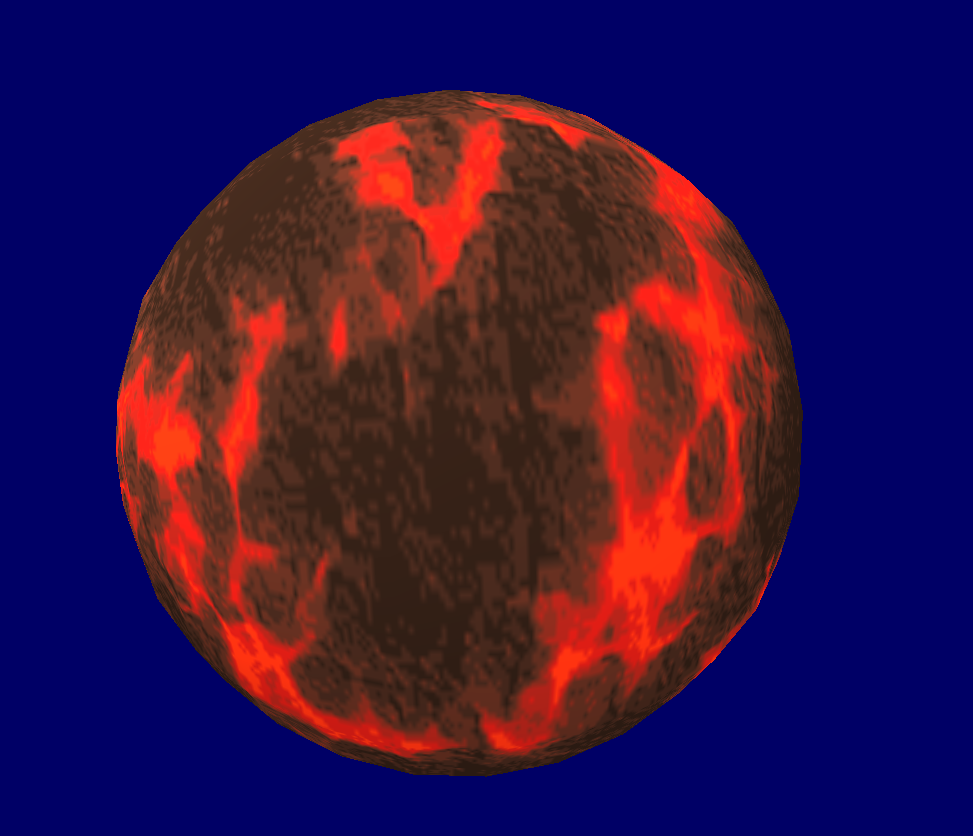
\includegraphics[scale=0.3]{sphereLava.png}
    \caption{Sphere avec texture lave}
\end{figure}

\newpage
\section{Plaquage d'une texture avec utilisation d'une normalMap}

On fait pareil que précédemment pour avoir une texture, mais on ajoute cette fois ci un autre objet texture qui est notre texture normalMap, en faisant exacatement pareil que précédement mais en donnant en paramètre de loadTexture2DFromFilePath la path de notre image normalMap.
Il faut pour cela calculer un rendu de lumière avec Phong, das le vertex shader, par exemple pour cela on utilise la normale, pour avoir la tangeante et la bitangeante puis dans le fragment shader on calcule notre phong en utilisant comme normal celle de notre texture NormalMap.
\begin{lstlisting}
	#version 330 core

out vec4 FragColor;

in vec3 o_positionWorld;
in vec2 o_uv0;
in vec3 tangentLightPos;
in vec3 tangentViewPos;
in vec3 tangentFragmentPos;

uniform sampler2D colorText;
uniform sampler2D normalText;
uniform vec3 lightPos;
uniform vec3 viewPos;

void main() {
    
    vec3 normal=texture(normalText,o_uv0).rgb;
    normal=normalize(normal*2.0-1.0);

    vec3 color=texture(colorText,o_uv0).rgb;

    vec3 ambiant=1.0*color;

    vec3 lightDir=normalize(tangentLightPos -tangentFragmentPos);
    float diff=max(dot(lightDir,normal),0.0);
    vec3 diffuse=diff*color;

    vec3 viewDir=normalize(tangentViewPos-tangentFragmentPos);
    vec3 reflex=reflect(-lightDir,normal);
    vec3 halfway=normalize(lightDir+viewDir);
    float spec=pow(max(dot(normal, halfway),0.0),32.0);
    vec3 specular=vec3(0.2)*spec;

    FragColor=vec4(ambiant+diffuse+specular,1.0);
}

\end{lstlisting}

\begin{figure}[h]
    \center
    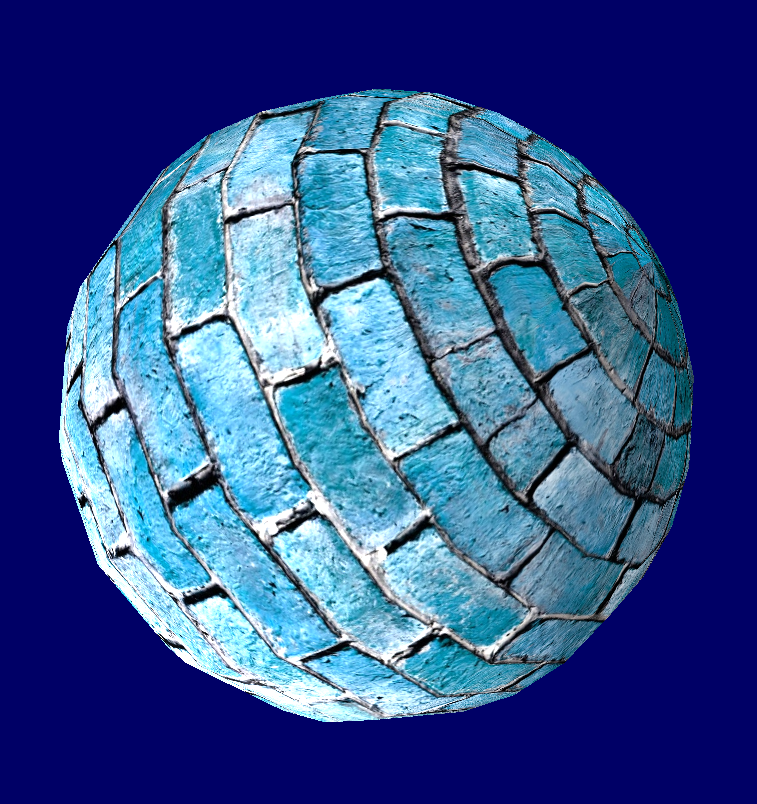
\includegraphics[scale=0.3]{sphereTexture.png}
    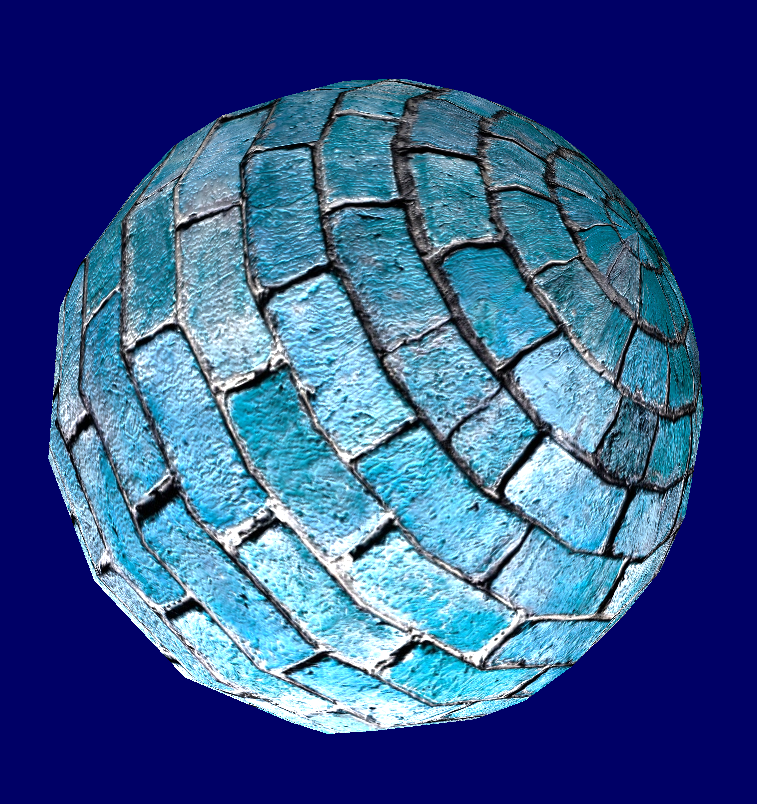
\includegraphics[scale=0.3]{sphereTextureNormalMap.png}
    \caption{Sphere avec texture brick, sans normalMap à gauche et avec normalMap à droite}
\end{figure}


\section{SkyBox}
Pour réaliser la skyBox on définit un objet vertex array sur notre GPU puis grâce à un buffer on lui envoi les données des vertices de notre cube.
Puis on créé et on load une texture cube (plusieurs images), et on envoi celle-ci au fragment shader, pour faire la même chose que pour une texture classique mais avec cette fois-ci une texture cube et des coordonées 3D.

\begin{lstlisting}

	//Material.cpp
	
	glGenVertexArrays(1, &skyboxVAO);
	glGenBuffers(1, &skyboxVBO);
	glBindVertexArray(skyboxVAO);
	glBindBuffer(GL_ARRAY_BUFFER, skyboxVBO);
	glBufferData(GL_ARRAY_BUFFER, sizeof(skyboxVertices), &skyboxVertices, GL_STATIC_DRAW);
	glEnableVertexAttribArray(0);
	glVertexAttribPointer(0, 3, GL_FLOAT, GL_FALSE, 3 * sizeof(float), (void *)0);

	m_texture = loadSkybox(faces);

	//Texture.cpp

	GLuint loadSkybox(std::vector<std::string> faces){
	GLuint texture;
	glGenTextures(1, &texture);
	glBindTexture(GL_TEXTURE_CUBE_MAP, texture);

	int width, height, nrChannels;
	unsigned char *data;
	for(unsigned int i=0; i<faces.size(); i++){
		//faces est un tableau de string contenant les chemins des images textures de la skybox 
		data = stbi_load(faces[i].c_str(), &width, &height, &nrChannels, 0);
		if(data){
			stbi_set_flip_vertically_on_load(false);
			glTexImage2D(GL_TEXTURE_CUBE_MAP_POSITIVE_X + i, 0, GL_RGB, width, height, 0, GL_RGB, GL_UNSIGNED_BYTE, data);
			stbi_image_free(data);
		}
		else{
			std::cout<<"ERROR!"<<std::endl;
			stbi_image_free(data);
		}
	}
	glTexParameteri(GL_TEXTURE_CUBE_MAP, GL_TEXTURE_MIN_FILTER, GL_LINEAR);
    glTexParameteri(GL_TEXTURE_CUBE_MAP, GL_TEXTURE_MAG_FILTER, GL_LINEAR);
    glTexParameteri(GL_TEXTURE_CUBE_MAP, GL_TEXTURE_WRAP_S, GL_CLAMP_TO_EDGE);
    glTexParameteri(GL_TEXTURE_CUBE_MAP, GL_TEXTURE_WRAP_T, GL_CLAMP_TO_EDGE);
    glTexParameteri(GL_TEXTURE_CUBE_MAP, GL_TEXTURE_WRAP_R, GL_CLAMP_TO_EDGE);

	return texture;
}

\end{lstlisting}

\begin{figure}[h]
    \center
    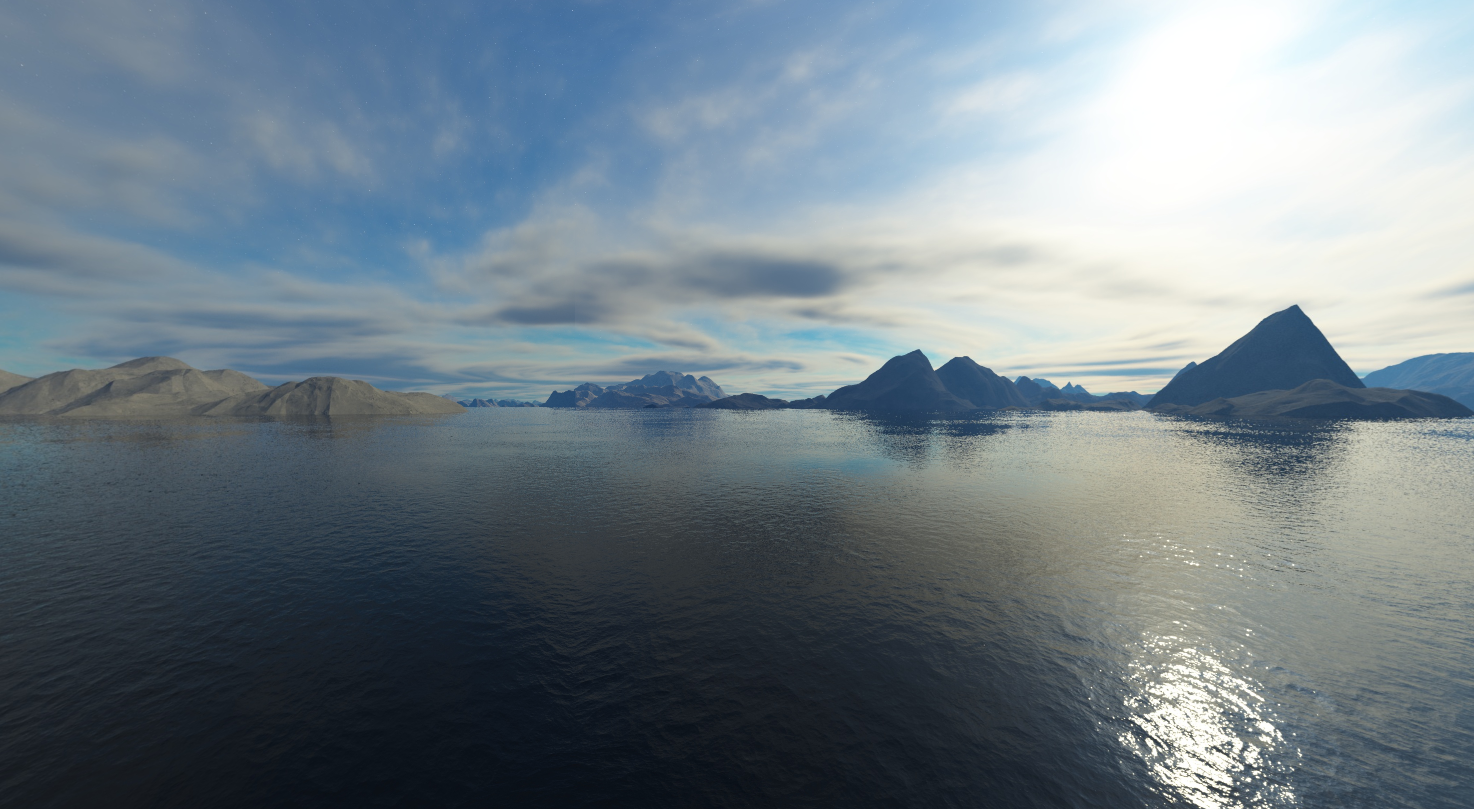
\includegraphics[scale=0.25]{skybox.png}
    \caption{Skybox}
\end{figure}

\section{Objet reflété}
Dans un premier temps il faut créer 2 couples de shader un qui gèrera la skybox et l'autre l'objet dans la skybox.
Pour cela on créé 2 programmes, et on rajoute un attribut à la fonction bind de material pour qu'il sache si il s'agit de la procédure pour la skybox ou pour l'objet on modifie l'id du program en fonction (pour cela j'ai utilisé un id utilisé et 2 autres qui correspondent aux 2 cas de figure et qui seront atribué selon le cas).

Pour le 2e couple de shader (celui de l'objet) on récupère la normale (en pensant à transformer les normales pour qu'elles soient adaptées aux transformations appliquées), on envoi la normale et la position au fragment shader qui lui calcule le rayon incident grâce à la position de la caméra. Avec la fonction reflex et en donnant en paramètre le rayon incident et la normale tout eux normalisés, cela nous donne le rayon de réflexion et on s'en sert pour récupérer la valeur du fragment à refléter.

\begin{lstlisting}
void Material::bind(bool cube)
{
	check();
	ObjetSkybox = cube;
	if (cube)
	{
		m_program = skyboxprogram;
	}
	else
	{
		m_program = sphereprogram;
	}
	glUseProgram(m_program);

	internalBind();
}


void Material::internalBind()
{
	// bind parameters

	if (ObjetSkybox && m_texture != -1)
	{
		glDepthMask(GL_FALSE);
		glDepthFunc(GL_LEQUAL);
		glBindVertexArray(skyboxVAO);
		glActiveTexture(GL_TEXTURE0);
		glBindTexture(GL_TEXTURE_CUBE_MAP, m_texture);
		glDrawArrays(GL_TRIANGLES, 0, 36);
		glBindVertexArray(0);
		glDepthFunc(GL_LESS);
		glDepthMask(GL_TRUE);
	}
	else if (m_textureSphere != -1)
	{
		glUniform1i(getUniform("Texture"), 0);
		glActiveTexture(GL_TEXTURE0);
		glBindTexture(GL_TEXTURE_CUBE_MAP, m_textureSphere);
	}
	GLuint c_p = glGetUniformLocation(sphereprogram, "cameraPos");
    glUniform3f(c_p,Context::camera.position[0], Context::camera.position[1], Context::camera.position[2]);

}

\end{lstlisting}


\begin{lstlisting}
//vertex shader

#version 330 core

layout(location = 0) in vec3 position;
layout(location = 1) in vec3 normal;
layout(location = 2) in vec2 texCoord;

uniform mat4 model;
uniform mat4 view;
uniform mat4 projection; 

out vec3 coordonneesText;
out vec3 normalText;

void main() {
  normalText=mat3(transpose(inverse(model)))*normal;
  coordonneesText=vec3(model*vec4(position,1.0));
  gl_Position = projection * view  * vec4(position.x,-position.y,-position.z,1.0);
}

//fragment shader

#version 330 core

out vec4 FragColor;

in vec3 coordonneesText;
in vec3 normalText;

uniform vec3 cameraPos;

uniform samplerCube Texture;

void main()
{             
    vec3 I = normalize(coordonneesText - cameraPos);
    vec3 R = reflect(I, normalize(normalText));
    FragColor = vec4(texture(Texture, R).rgb, 1.0);
}
\end{lstlisting}


\begin{figure}[h]
    \center
    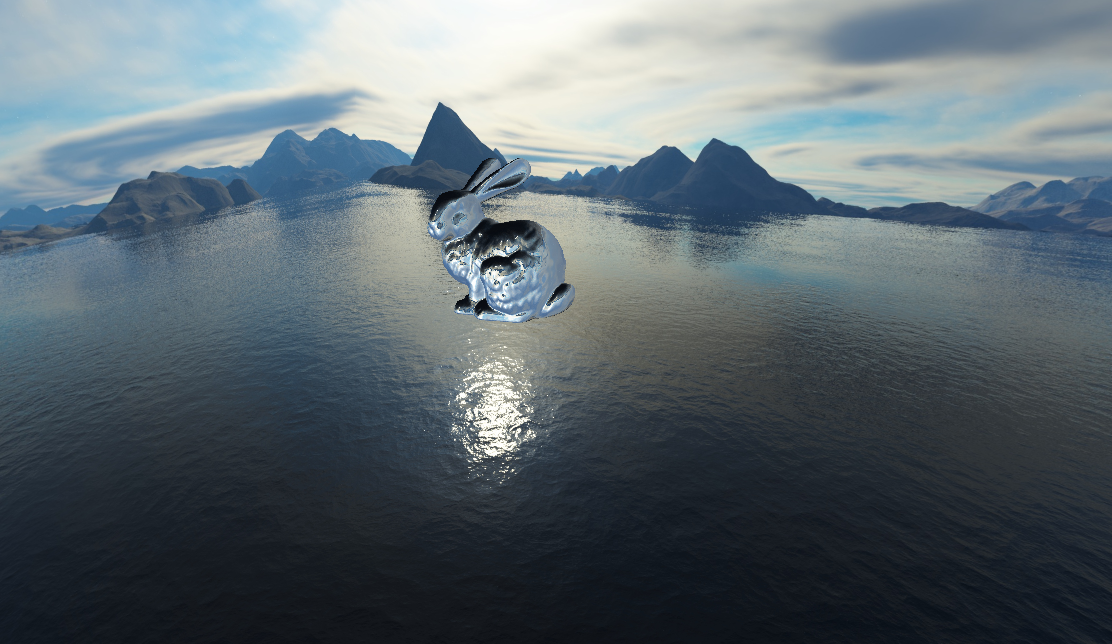
\includegraphics[scale=0.3]{skyboxObjReflex.png}
    \caption{Skybox avec objet reflété}
\end{figure}



\section{Remarques}

Ce Tp était assez long et assez compliqué à comprendre bien qu'on maitrisait les différents éléments utilisés comme les shaders ou les buffers, des choses précisent comme l'utilisation de 2 shaders.
Le conseil de l'utilisation de LearOpenGL a été très utile.

Cependant long et peu de temps avec les autres travaux et les révisions je n'ai pas eu le temps d'aborder le second TP.


\end{document}